
\chapter{ANALYSE ET SPÉCIFICATION DES BESOINS}

\section*{Introduction}
\addcontentsline{toc}{section}{Introduction}

La réussite technique du \textit{HydroNova} repose sur une définition précise des attentes des utilisateurs et des exigences opérationnelles des machines. Ce chapitre détaille l'analyse des besoins en segmentant le système en quatre piliers technologiques : l'application mobile pour l'exploitant, l'interface web pour l'administration, l'infrastructure IoT pour le contrôle local, et l'intelligence artificielle pour le diagnostic sanitaire. Cette approche permet de garantir que chaque composant répond aux standards de performance et de fiabilité requis.

%================================================================
\section{Identification des Acteurs}
%================================================================

La conception d’un écosystème IoT intelligent et décentralisé nécessite une identification claire des différentes entités interagissant avec le système. Les acteurs représentent aussi bien les utilisateurs humains que les composants logiciels et matériels capables d’échanger des données ou d’exécuter des traitements autonomes.

Dans le cadre de ce projet, les acteurs sont répartis en deux catégories principales : les acteurs humains et les acteurs systémiques.


\subsection{Acteurs}

\begin{itemize}
	\item \textbf{L'Agriculteur :} Acteur principal du système et utilisateur final de l’application mobile. Il supervise les paramètres environnementaux de la serre, contrôle les équipements connectés, suit les cycles de production et exploite les outils d’assistance intelligente afin d’optimiser la production hydroponique.
	
	\item \textbf{Visiteur :} Utilisateur disposant d’un accès restreint à certaines fonctionnalités publiques de la plateforme. Il peut interagir avec le chatbot intelligent, consulter les actualités agricole .
	
	\item \textbf{L'Administrateur :} Responsable de la gestion globale de la plateforme via l’interface web d’administration. Il supervise les utilisateurs, les serres déployées, les configurations système, les droits d’accès ainsi que les opérations de maintenance et de supervision centralisée.
	
	\item \textbf{Agent Technique :} Technicien chargé des interventions techniques sur les équipements déployés. Il assure les opérations de maintenance corrective et préventive .
\end{itemize}
    %================================================================
\section{Spécification des Besoins}
%================================================================

Après l’identification des acteurs, cette section formalise les besoins fonctionnels et non fonctionnels du système. L’analyse est structurée autour des quatre piliers technologiques de la plateforme : le sous-système mobile destiné à l’exploitant, le sous-système web dédié à l’administration, le sous-système IoT assurant le contrôle local, et le sous-système d’intelligence artificielle responsable du diagnostic sanitaire.

\subsection{Sous-système Mobile}
Cette section présente les besoins fonctionnels et non fonctionnels de l’application mobile du système.
Elle décrit les principales fonctionnalités offertes aux différents types d’utilisateurs ainsi que les contraintes garantissant la qualité du service.
\subsubsection{Besoins Fonctionnels}

\begingroup
\footnotesize % Taille de police légèrement réduite pour gagner de l'espace
\setlength{\tabcolsep}{4pt} % Réduction des marges intérieures des colonnes (défaut : 6pt)
\renewcommand{\arraystretch}{1.2} % Espacement vertical plus compact et adapté au texte multiligne

\begin{longtable}{|p{0.24\textwidth}|>{\raggedright\arraybackslash}p{0.54\textwidth}|>{\raggedright\arraybackslash}p{0.16\textwidth}|}
	\hline
	\rowcolor[HTML]{2C3E50}
	\textcolor{white}{\textbf{Besoin}} &
	\textcolor{white}{\textbf{Description}} &
	\textcolor{white}{\textbf{Acteur Concerné}} \\ \hline
	\endfirsthead
	
	\hline
	\rowcolor[HTML]{2C3E50}
	\textcolor{white}{\textbf{Besoin}} &
	\textcolor{white}{\textbf{Description}} &
	\textcolor{white}{\textbf{Acteur Concerné}} \\ \hline
	\endhead
	
	\textbf{Authentification et gestion de compte} &
	Le système doit permettre aux utilisateurs de créer un compte et de s’authentifier de manière sécurisée avec gestion des accès. &
	Agriculteur, Visiteur \\ \hline
	
	\textbf{Supervision de la serre} &
	Le système doit permettre la consultation en temps réel des données environnementales de la serre. &
	Agriculteur \\ \hline
	
	\textbf{Contrôle des équipements de la serre} &
	Le système doit permettre le contrôle manuel des équipements tels que l’irrigation, l’éclairage et la ventilation ... &
	Agriculteur \\ \hline
	
	\textbf{Analyse et historique des cultures} &
	Le système doit permettre la consultation des statistiques et de l’historique des cycles de production afin de suivre l’évolution des cultures. &
	Agriculteur \\ \hline
	
	\textbf{Assistance intelligente multilingue (Chatbot)} &
	Le système doit intégrer un chatbot intelligent capable d’assister les utilisateurs en plusieurs langues et de répondre aux questions liées à l’hydroponie et à la plateforme. &
	Agriculteur, Visiteur \\ \hline
	
	\textbf{Notifications et alertes de la serre} &
	Le système doit envoyer à l’agriculteur des notifications liées aux anomalies détectées, aux alertes critiques issues des capteurs . &
	Agriculteur \\ \hline
	
	\textbf{Notifications de contenu et actualités} &
	Le système doit envoyer aux visiteurs des notifications concernant les nouvelles publications, les actualités agricoles et les mises à jour de la plateforme. &
	Visiteur \\ \hline
	
	\textbf{Abonnement aux mises à jour} &
	Le système doit permettre aux visiteurs de s’abonner afin de recevoir des notifications personnalisées liées aux contenus agricoles, au chatbot et aux nouvelles fonctionnalités de la plateforme. &
	Visiteur \\ \hline
	
	\caption{Besoins fonctionnels de l’application mobile}
	\label{tab:bf-mobile}
\end{longtable}
\endgroup
\subsubsection{Besoins Non Fonctionnels}


\begingroup
\footnotesize % Taille de police légèrement réduite pour gagner de l'espace
\setlength{\tabcolsep}{4pt} % Réduction des marges intérieures des colonnes
\renewcommand{\arraystretch}{1.2} % Espacement vertical plus compact et adapté au texte multiligne

\begin{longtable}{|>{\raggedright\arraybackslash}p{4cm}|>{\raggedright\arraybackslash}p{10cm}|}
	\hline
	\rowcolor[HTML]{2C3E50}
	\textcolor{white}{\textbf{Critère}} & \textcolor{white}{\textbf{Exigence Technique}}
	\\ \hline
	\endfirsthead
	
	\hline
	\rowcolor[HTML]{2C3E50}
	\textcolor{white}{\textbf{Critère}} & \textcolor{white}{\textbf{Exigence Technique}}
	\\ \hline
	\endhead
	
	\textbf{Performance} &
	L’application mobile doit garantir une faible latence dans l’affichage des données critiques afin d’assurer une expérience utilisateur fluide et réactive.
	\\ \hline
	
	\textbf{Réactivité} &
	L’interface doit rester fluide même en cas de forte charge, avec une gestion optimisée des mises à jour via un mécanismes équivalents.
	\\ \hline
	
	\textbf{Disponibilité} &
	Le système doit assurer une disponibilité continue des fonctionnalités essentielles. 
	\\ \hline
	
	\textbf{Sécurité} &
	L’accès à l’application doit être sécurisé par authentification , avec chiffrement des échanges entre le client mobile et le backend.
	\\ \hline
	
	\textbf{Ergonomie} &
	L’interface utilisateur doit être intuitive, responsive et adaptée à une utilisation sur le terrain, même dans des conditions d’usage difficiles.
	\\ \hline
	
	\textbf{Compatibilité} &
	L’application doit être compatible avec les systèmes Android et iOS, garantissant une expérience utilisateur homogène sur différentes plateformes.
	\\ \hline
	
	\textbf{Scalabilité} &
	L’architecture doit permettre la montée en charge du nombre d’utilisateurs et de serres connectées sans dégradation notable des performances.
	\\ \hline
	
	\textbf{Robustesse} &
	Le système doit rester fonctionnel en cas de coupures réseau intermittentes, avec synchronisation automatique lors de la reconnexion.
	\\ \hline
	
	\caption{Besoins non fonctionnels de l’application mobile}
	\label{tab:nf-mobile}
\end{longtable}
\endgroup
%================================================================

%----------------------------------------------------------------
\subsection{Sous-système Web}

Cette section présente les besoins fonctionnels et non fonctionnels du sous-système web de la plateforme.  
Elle décrit les fonctionnalités dédiées à la supervision, à la gestion du système ainsi qu’à l’administration des équipements et des utilisateurs.
\subsubsection{Besoins Fonctionnels}

\begingroup
\footnotesize % Taille de police légèrement réduite pour gagner de l'espace
\setlength{\tabcolsep}{4pt} % Réduction des marges intérieures des colonnes
\renewcommand{\arraystretch}{1.5} % Espacement vertical choisi

{\small
	\renewcommand{\arraystretch}{1.5}
	\begin{longtable}{|>{\raggedright\arraybackslash}p{4cm}|>{\raggedright\arraybackslash}p{9cm}|>{\raggedright\arraybackslash}p{3cm}|}
		
		\hline
		\rowcolor[HTML]{2C3E50}
		\textcolor{white}{\textbf{Besoin}} &
		\textcolor{white}{\textbf{Description}} &
		\textcolor{white}{\textbf{Acteur Concerné}}
		\\ \hline
		\endfirsthead
		
		\hline
		\rowcolor[HTML]{2C3E50}
		\textcolor{white}{\textbf{Besoin}} &
		\textcolor{white}{\textbf{Description}} &
		\textcolor{white}{\textbf{Acteur Concerné}}
		\\ \hline
		\endhead
		
		\rowcolor[HTML]{EFEFEF}
		\textbf{Gestion des comptes utilisateurs} &
		Le système doit permettre la création, la modification, la suspension et la suppression des comptes utilisateurs. &
		Administrateur
		\\ \hline
		
		\textbf{Gestion des rôles et permissions (RBAC)} &
		Le système doit permettre la définition et la gestion des rôles ainsi que des droits d’accès selon les profils utilisateurs. &
		Administrateur
		\\ \hline
		
		\rowcolor[HTML]{EFEFEF}
		\textbf{Supervision globale des serres} &
		Le système doit fournir une vue centralisée de l’état des serres et des équipements connectés. &
		Administrateur, Agent Technique
		\\ \hline
		
		\textbf{Gestion des équipements IoT} &
		Le système doit permettre l’enregistrement, la configuration et la supervision des capteurs et actionneurs installés dans les serres. &
		Agent Technique
		\\ \hline
		
		\rowcolor[HTML]{EFEFEF}
		\textbf{Analyse et statistiques globales} &
		Le système doit fournir des tableaux de bord analytiques permettant le suivi des performances de la plateforme et des serres. &
		Administrateur
		\\ \hline
		
		\textbf{Gestion des contenus et actualités} &
		Le système doit permettre la création, la modification et la publication d’articles destinés aux utilisateurs de la plateforme. &
		Administrateur
		\\ \hline
		
		\rowcolor[HTML]{EFEFEF}
		
		
		\textbf{Gestion des interventions techniques} &
		Le système doit permettre la création, la consultation et le suivi des tickets d’intervention liés aux équipements des serres. &
		Agent Technique
		\\ \hline
		
		\rowcolor[HTML]{EFEFEF}
		
		
		\textbf{Déploiement des mises à jour} &
		Le système doit permettre la mise à jour à distance des équipements, capteurs, actionneurs et modules logiciels. &
		Agent Technique
		\\ \hline
		
		\caption{Besoins fonctionnels de l’application web (Administrateur et Agent Technique)}
		\label{tab:bf-web-combined}
		
	\end{longtable}
}
\endgroup
% ==========================================================
\subsubsection{Besoins Non Fonctionnels}

\renewcommand{\arraystretch}{1.5}

{\small
	\renewcommand{\arraystretch}{1.5}
	\begin{longtable}{|p{4cm}|p{9cm}|}
		
		\hline
		\rowcolor[HTML]{2C3E50}
		\textcolor{white}{\textbf{Critère}} &
		\textcolor{white}{\textbf{Exigence}}
		\\ \hline
		\endfirsthead
		
		\hline
		\rowcolor[HTML]{2C3E50}
		\textcolor{white}{\textbf{Critère}} &
		\textcolor{white}{\textbf{Exigence}}
		\\ \hline
		\endhead
		
		\rowcolor[HTML]{EFEFEF}
		\textbf{Scalabilité} &
		Le système doit supporter l’augmentation du nombre de serres et d’utilisateurs sans dégradation des performances.
		\\ \hline
		
		\textbf{Fiabilité} &
		Le système doit garantir l’intégrité et la cohérence des données enregistrées.
		\\ \hline
		
		\rowcolor[HTML]{EFEFEF}
		\textbf{Sécurité renforcée} &
		Les opérations critiques doivent être protégées par des mécanismes de sécurité avancés.
		\\ \hline
		
		\textbf{Performance} &
		L’interface web doit offrir des temps de chargement rapides afin d’améliorer la productivité des utilisateurs.
		\\ \hline
		
		\rowcolor[HTML]{EFEFEF}
		\textbf{Traçabilité} &
		Toutes les opérations importantes doivent être journalisées afin de faciliter les audits et la maintenance.
		\\ \hline
		
		\caption{Besoins non fonctionnels de l’interface web}
		\label{tab:bnf-web}
		
	\end{longtable}
}
%----------------------------------------------------------------
\subsection{Sous-système IoT}

Le système embarqué constitue le cœur opérationnel de la serre intelligente. Il assure le contrôle local des équipements ainsi que la collecte des données en périphérie (Edge Computing), garantissant ainsi l’autonomie du système même en cas de perte de connectivité.

% ==========================================================
\subsubsection{Besoins Fonctionnels}

{\small
	\renewcommand{\arraystretch}{1.5}
	\begin{longtable}{|p{4cm}|p{9cm}|}

		\hline
		\rowcolor[HTML]{2C3E50}
		\textcolor{white}{\textbf{Besoin}} &
		\textcolor{white}{\textbf{Description}}
		\\ \hline
		\endfirsthead

		\hline
		\rowcolor[HTML]{2C3E50}
		\textcolor{white}{\textbf{Besoin}} &
		\textcolor{white}{\textbf{Description}}
		\\ \hline
		\endhead

		\rowcolor[HTML]{EFEFEF}
		\textbf{Collecte des données environnementales} &
		Le système doit assurer l’acquisition continue et périodique des données provenant des capteurs environnementaux (température, humidité, CO2 ...). 
		\\ \hline
		
		\textbf{Communication IoT avec le backend} &
		Le système doit transmettre les données télémétriques vers le backend et recevoir les commandes de contrôle des équipements de la serre. 
		\\ \hline
		
		\rowcolor[HTML]{EFEFEF}
		\textbf{Contrôle autonome de la serre} &
		Le système doit garantir le fonctionnement des équipements critiques (irrigation, ventilation, détection de maladie , ... ) de manière autonome en cas de perte de connexion réseau. 
		\\ \hline
		
		\textbf{Synchronisation des données locales} &
		Le système doit synchroniser automatiquement les données stockées localement avec le backend dès le rétablissement de la connexion réseau. 
		\\ \hline
		
		\caption{Besoins fonctionnels du système embarqué}
		\label{tab:bf-embedded}
		
	\end{longtable}
}
% ==========================================================
\subsubsection{Besoins Non Fonctionnels}

\renewcommand{\arraystretch}{1.5}

{\small
	\renewcommand{\arraystretch}{1.5}
	\begin{longtable}{|p{4cm}|p{9cm}|}
		
		\hline
		\rowcolor[HTML]{2C3E50}
		\textcolor{white}{\textbf{Critère}} &
		\textcolor{white}{\textbf{Exigence}}
		\\ \hline
		\endfirsthead
		
		\hline
		\rowcolor[HTML]{2C3E50}
		\textcolor{white}{\textbf{Critère}} &
		\textcolor{white}{\textbf{Exigence}}
		\\ \hline
		\endhead
		
		\rowcolor[HTML]{EFEFEF}
		\textbf{Disponibilité} &
		Le système embarqué doit garantir un fonctionnement continu afin d’assurer la survie des cultures et la stabilité de la serre.
		\\ \hline
		
		\textbf{Optimisation des ressources} &
		Le système doit limiter la consommation mémoire et CPU afin de rester compatible avec les capacités matérielles du matériel embarqué.
		\\ \hline
		
		\caption{Besoins non fonctionnels du système embarqué}
		\label{tab:bnf-embedded}
		
	\end{longtable}
}

%----------------------------------------------------------------
\subsection{Sous-système d'Intelligence Artificielle}

Le sous-système d’intelligence artificielle constitue le module central chargé de l’analyse automatique des données visuelles et de la détection des anomalies phytosanitaires.

% ==========================================================
\subsubsection{Besoins Fonctionnels}

{\small
	\renewcommand{\arraystretch}{1.5}
	\begin{longtable}{|p{4cm}|p{9cm}|}
		
		\hline
		\rowcolor[HTML]{2C3E50}
		\textcolor{white}{\textbf{Besoin}} &
		\textcolor{white}{\textbf{Description}}
		\\ \hline
		\endfirsthead
		
		\hline
		\rowcolor[HTML]{2C3E50}
		\textcolor{white}{\textbf{Besoin}} &
		\textcolor{white}{\textbf{Description}}
		\\ \hline
		\endhead
		
		\rowcolor[HTML]{EFEFEF}
		\textbf{Analyse intelligente des images (Edge AI)} &
		Le module d’intelligence artificielle doit analyser localement les images capturées afin de détecter les maladies, carences et anomalies affectant les cultures. 
		\\ \hline
		

		
		
		\caption{Besoins fonctionnels du module IA}
		\label{tab:bf-ia}
		
	\end{longtable}
}
% ==========================================================
\subsubsection{Besoins Non Fonctionnels}

\renewcommand{\arraystretch}{1.5}

{\small
	\renewcommand{\arraystretch}{1.5}
	\begin{longtable}{|p{4cm}|p{9cm}|}
		
		\hline
		\rowcolor[HTML]{2C3E50}
		\textcolor{white}{\textbf{Critère}} &
		\textcolor{white}{\textbf{Exigence}}
		\\ \hline
		\endfirsthead
		
		\hline
		\rowcolor[HTML]{2C3E50}
		\textcolor{white}{\textbf{Critère}} &
		\textcolor{white}{\textbf{Exigence}}
		\\ \hline
        
		\endhead
		\rowcolor[HTML]{EFEFEF}
		\textbf{Certitude des prédictions} &
		Le modèle d'IA doit bien connaître les caractéristiques des maladies afin de garantir un niveau de certitude élevé lors des détections.
		\\ \hline

		\caption{Besoins non fonctionnels du module IA}
		\label{tab:bnf-ia}
		
	\end{longtable}
}
Ainsi, afin de représenter de manière claire, structurée et normalisée les besoins fonctionnels et non fonctionnels du système, il est nécessaire d’adopter un langage de modélisation adapté à la conception et à la formalisation de l’architecture logicielle.

%================================================================
\sectiontitle{Langage de modélisation}
%================================================================

Dans le cadre de ce projet, la définition des besoins et la conception du système nécessitent une représentation standardisée et compréhensible par l’ensemble des parties prenantes. Pour cela, nous avons retenu le langage UML (Unified Modeling Language), qui constitue aujourd’hui un standard incontournable dans le domaine du génie logiciel.

L’UML est un langage graphique basé sur un ensemble de diagrammes permettant de représenter visuellement la structure statique et le comportement dynamique d’un système. Il est largement utilisé dans les projets orientés objet, mais peut également être appliqué à d’autres domaines nécessitant une modélisation claire et structurée.

\subsectiontitle{Pourquoi utiliser UML ?}

L’UML est un langage formel et standardisé qui facilite la modélisation des systèmes complexes. Son principal avantage réside dans son indépendance vis-à-vis des langages de programmation, ce qui en fait un outil universel de conception.

Il permet avant tout d’assurer une meilleure communication entre les différents acteurs d’un projet (développeurs, concepteurs, décideurs) grâce à une représentation visuelle commune et normalisée. Cette formalisation contribue à réduire les ambiguïtés, à améliorer la compréhension des besoins et à garantir une meilleure cohérence globale de la conception.

Dans ce chapitre, UML est utilisé comme support principal pour la modélisation des cas d’utilisation et la spécification des besoins du système.



\subsectiontitle{Dynamique Globale des Cas d'Utilisation}

Le diagramme des cas d'utilisation permet de définir les frontières fonctionnelles du système en identifiant les différents acteurs ainsi que les interactions qu’ils peuvent effectuer avec la plateforme. Il met en évidence les flux opérationnels autorisés pour chaque acteur et précise les responsabilités associées au système.

La représentation globale de ces interactions est illustrée par le diagramme suivant :



Comme le montre la figure~\ref{fig:usekbir}, le système est structuré autour de plusieurs acteurs et cas d’utilisation, permettant de visualiser clairement les fonctionnalités offertes ainsi que les échanges entre les différentes entités.
\begin{figure}[!h]
	\centering
	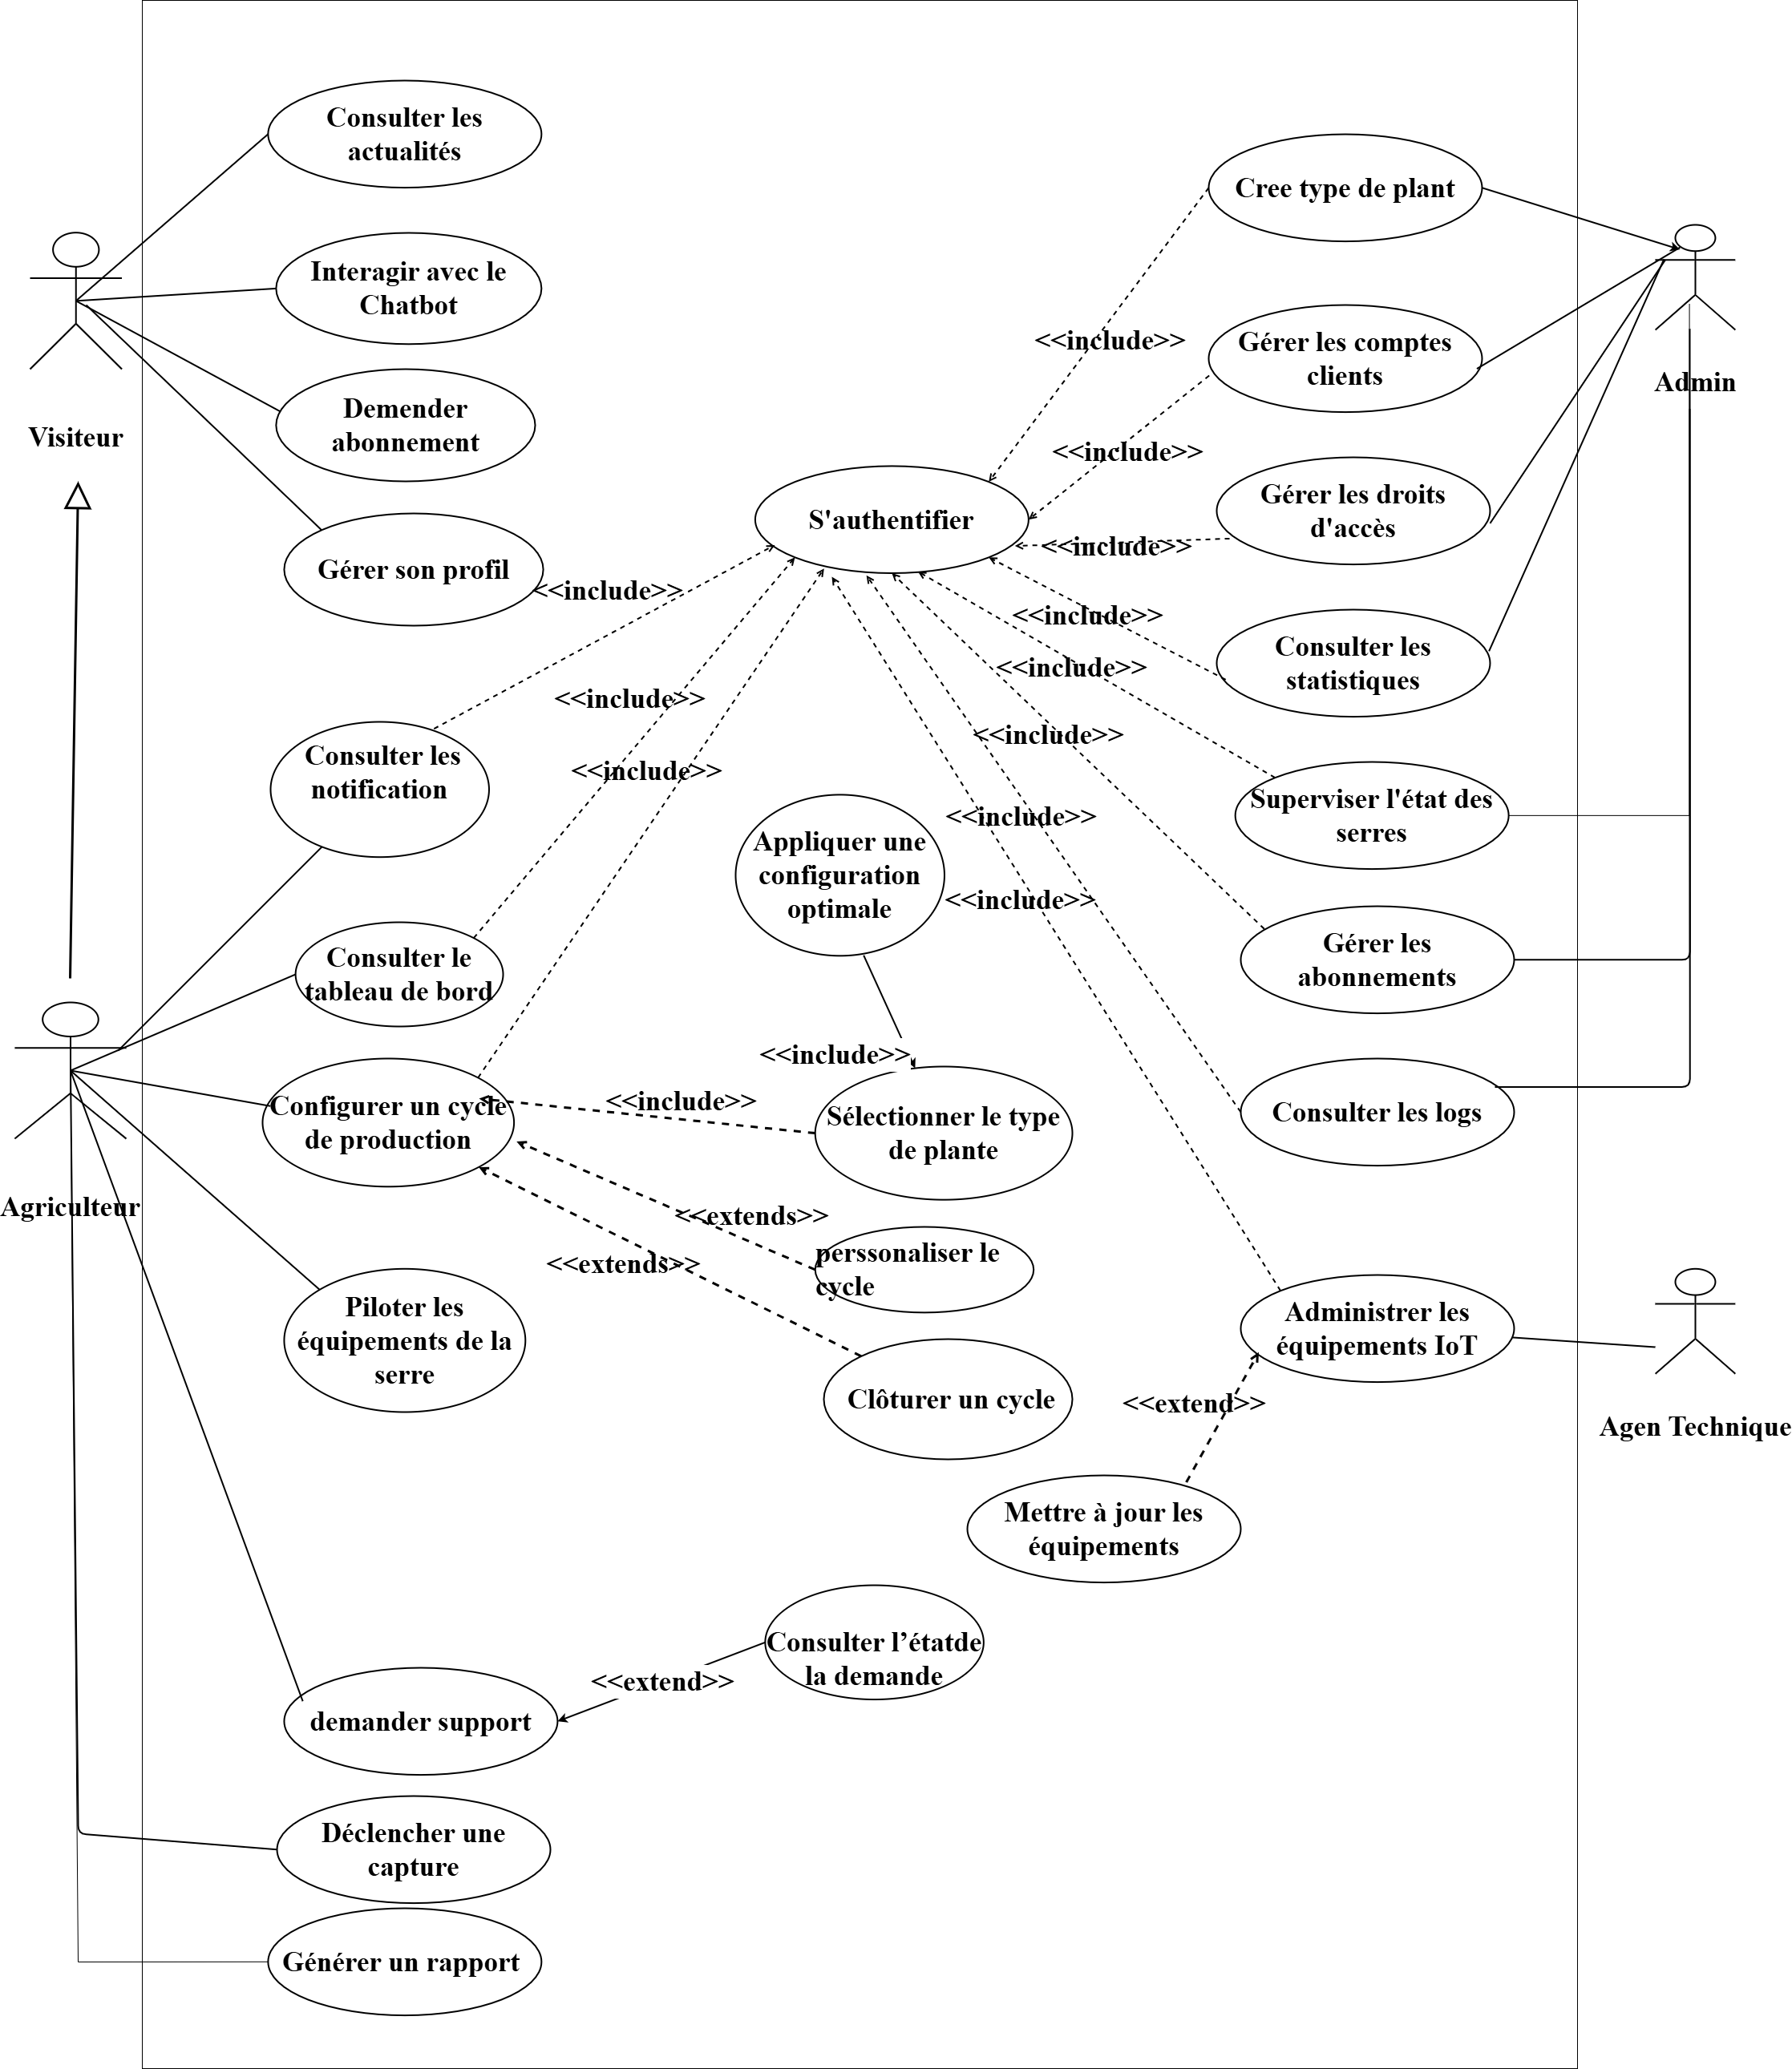
\includegraphics[width=1\linewidth]{public/casecase.drawio.png}
	\caption{Diagramme des cas d’utilisation du système}
	\label{fig:usekbir}
\end{figure}
\subsectiontitle{Diagramme de classe}
Le diagramme de classe métier présenté par la figure~\ref{fig:classanlse} décrit les entités clés intervenant dans le fonctionnement du système ainsi que leurs associations.
\begin{landscape} % active le mode paysage
\begin{figure}[tbph!]
	\centering
	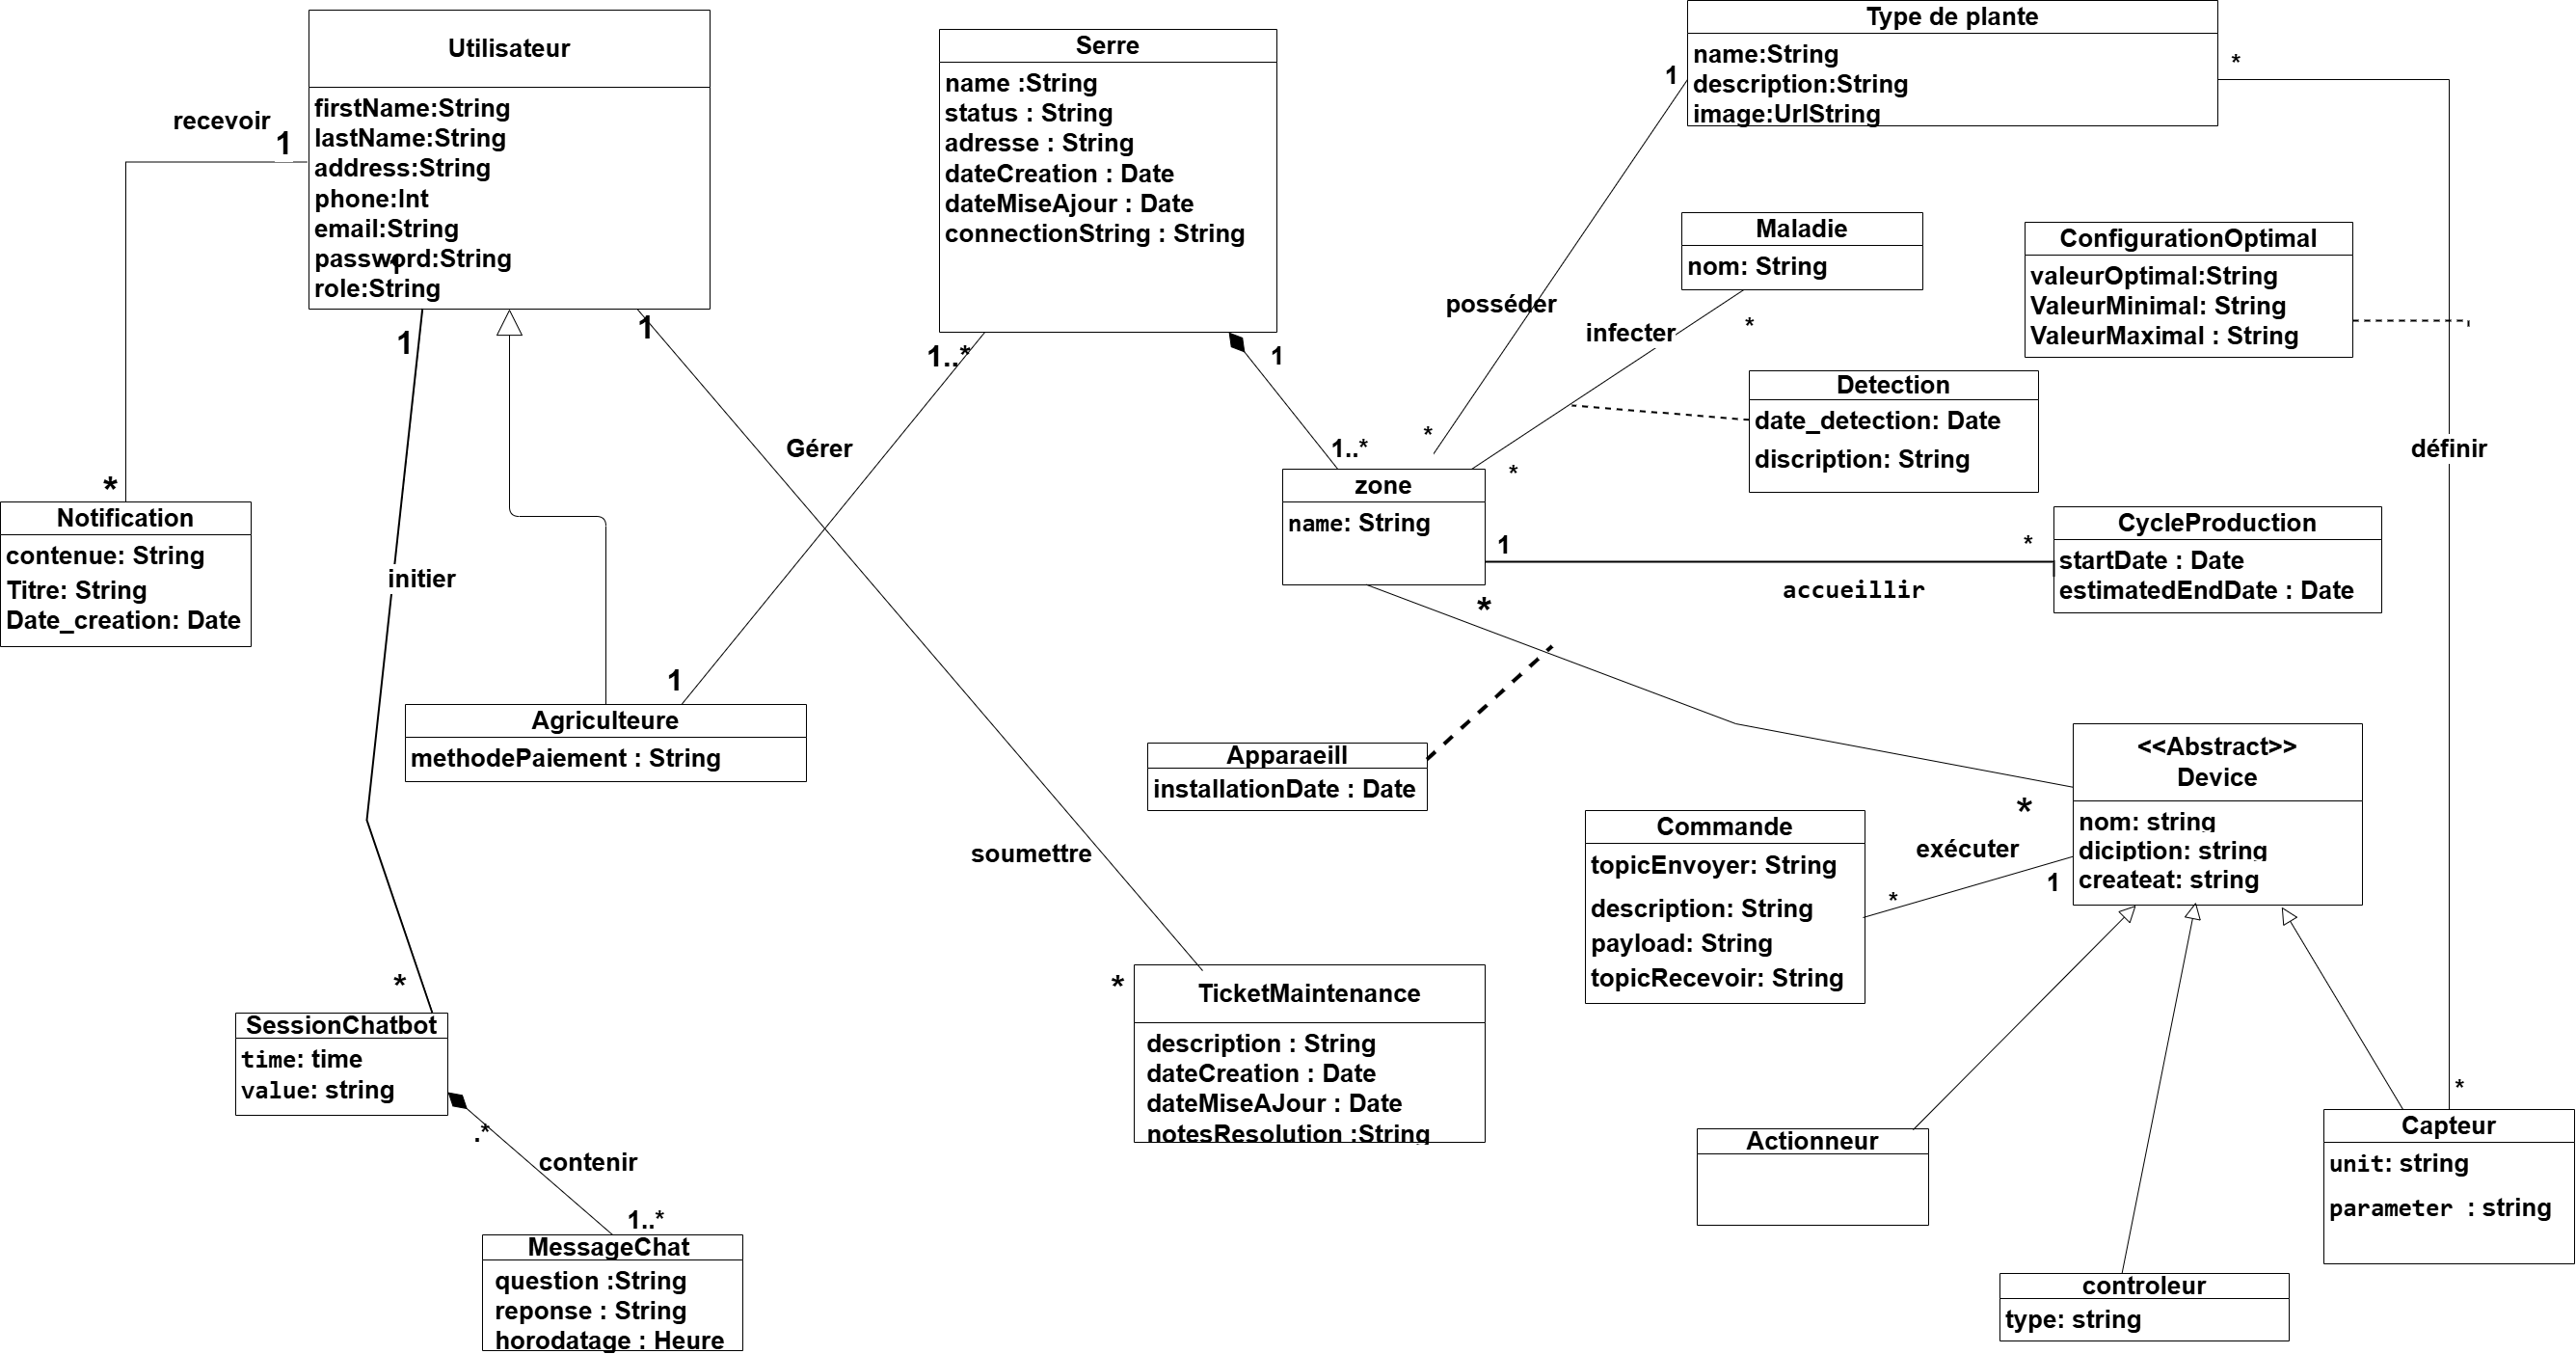
\includegraphics[width=1\linewidth]{public/classy.drawio}
	\caption{Diagramme de classes Analyse}
	\label{fig:classanlse}
\end{figure}
\end{landscape}

\section*{Conclusion}
\addcontentsline{toc}{section}{Conclusion}

Ce chapitre a permis de formaliser l’analyse et la spécification des besoins du système \textit{HydroNova}. Après avoir identifié les différents acteurs intervenant dans la plateforme, nous avons recensé de manière structurée les besoins fonctionnels et non fonctionnels propres à chacun des quatre sous-systèmes : l’application mobile de l’exploitant, l’interface web d’administration, l’infrastructure IoT embarquée et le module d’intelligence artificielle.

Cette spécification a ensuite été consolidée par une modélisation UML, à travers le diagramme des cas d’utilisation et le diagramme de classes, offrant une représentation claire et normalisée des interactions et des entités du système. L’ensemble constitue une base rigoureuse garantissant la traçabilité entre les exigences exprimées et les choix techniques à venir.

Les besoins étant désormais clairement établis et formalisés, le chapitre suivant aborde la phase de conception. Il détaillera l’architecture globale de la solution ainsi que les choix de conception adoptés afin de répondre aux exigences fonctionnelles et non fonctionnelles identifiées dans ce chapitre.